\documentclass{beamer}

\usetheme[subsection page=progressbar,progressbar=frametitle]{metropolis}
\usepackage{appendixnumberbeamer}

\usepackage{amsmath}
\usepackage{amssymb}
\usepackage{amsthm}
\usepackage{mathtools}
\usepackage{bussproofs}
\usepackage{stmaryrd}
\usepackage{gb4e}
\noautomath
\usepackage{url}
\usepackage{subcaption}
\usepackage{array}
\usepackage[toc,page]{appendix}
\usepackage[export]{adjustbox}[2011/08/13]
\usepackage{rotating}
\usepackage{tikz}
\usepackage{tikz-qtree}
\usepackage{etoolbox}
\usepackage{chngpage}
\usepackage{fancybox}
\usepackage{enumerate}
\usepackage{drs}
\input{qobitree}
\usepackage{forest}
\usepackage{color}
\usepackage{graphicx}

\newcommand{\hsbind}{\mathbin{\gg\!=}}
\newcommand{\apl}{\mathbin{\ll\!\!\cdot}}
\newcommand{\apr}{\mathbin{\cdot\!\!\gg}}
\newcommand{\aplr}{\mathbin{\ll\!\!\cdot\!\!\gg}}
\newcommand{\cons}{\mathbin{::}}
\newcommand{\cat}{\mathbin{+\mkern-10mu+}}

\newcommand{\abs}[1]{\textsc{#1}}
\newcommand{\obj}[1]{\textbf{#1}}
\newcommand{\sem}[1]{\llbracket #1 \rrbracket}
\newcommand{\lex}[2]{\sem{\abs{#1}} &:= #2}

\newcommand{\dand}{\mathbin{\overline{\land}}}
\newcommand{\dnot}{\mathop{\overline{\lnot}}}
\newcommand{\dor}{\mathop{\overline{\lor}}}
\newcommand{\dimpl}{\mathbin{\overline{\to}}}
\newcommand{\dexists}{\mathop{\overline{\exists}}}
\newcommand{\dforall}{\mathop{\overline{\forall}}}

\newcommand{\limp}{\mathbin{{-}\mkern-3.5mu{\circ}}}

\newcommand{\llbparenthesis}{\vcenter{\hbox{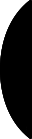
\includegraphics{symbols/llbparenthesis.png}}}}
\newcommand{\rrbparenthesis}{\vcenter{\hbox{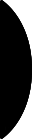
\includegraphics{symbols/rrbparenthesis.png}}}}
\newcommand{\lban}{\llparenthesis \,}
\newcommand{\rban}{\, \rrparenthesis}
\newcommand{\lbban}{\llbparenthesis \,}
\newcommand{\rbban}{\, \rrbparenthesis}
\newcommand{\banana}[1]{\lban #1 \rban}
\newcommand{\bbanana}[1]{\lbban #1 \rbban}
\newcommand{\cherry}{\rotatebox[origin=c]{270}{$\limp$}}

\newcommand{\lam}[2]{\lambda #1.\, #2}
\newcommand{\ap}[2]{#1\,#2}
\newcommand{\app}[3]{\ap{\ap{#1}{#2}}{#3}}
\newcommand{\appp}[4]{\ap{\ap{\ap{#1}{#2}}{#3}}{#4}}
\newcommand{\op}[1]{\mathtt{#1}}
\newcommand{\onto}[1]{#1 \mathalpha{:\,}}
\newcommand{\typedop}[3]{\op{#1} : #2 \rightarrowtail #3}
\newcommand{\typedopg}[3]{#1 : #2 \rightarrowtail #3}
\newcommand{\row}[2]{\{ #1 \mathrel{|} #2 \}}

\newcommand{\CC}{\mathcal{C}}
\newcommand{\FF}{\mathcal{F}}
\newcommand{\XX}{\mathcal{X}}
\newcommand{\EE}{\mathcal{E}}
\newcommand{\TT}{\mathcal{T}}
\newcommand{\PP}{\mathcal{P}}

\newcommand{\FV}{\operatorname{FV}}

\newcommand{\subst}[3]{#1[#2 \coloneqq #3]}

\newcommand{\syntclos}[1]{\mathbin{[#1]}}

\newcommand{\cibanana}{\banana{(\onto{\op{op}_i} M_i)_{i \in I},\ \onto{\eta} M_\eta}}
\newcommand{\cdbanana}{\banana{\onto{\op{op}_1} M_1,\ \dots,\ \onto{\op{op}_n} M_n,\ \onto{\eta} M_\eta}}

\newcommand{\cibbanana}{\bbanana{(\onto{\op{op}_i} M_i)_{i \in I},\ \onto{\eta} M_\eta}}

\newcommand{\TODO}[1]{\textbf{TODO}: #1}

\newcommand{\relR}{\mathbin{R}}

\newcommand{\swap}{\mathbin{\textbf{swap}}}

\newcommand{\tto}{\twoheadrightarrow}

\mathchardef\mhyphen="2D

\newcommand{\pair}[2]{\left<#1, #2\right>}
\newcommand{\inl}{\operatorname{inl}}
\newcommand{\inr}{\operatorname{inr}}

\newcommand{\true}{\textbf{T}}
\newcommand{\false}{\textbf{F}}
\newcommand{\ifte}[3]{\text{\textbf{if} $#1$ \textbf{then} $#2$ \textbf{else} $#3$}}


% Examples
\newcommand{\expr}[1]{\textsc{#1}}
\newcommand{\sume}{\expr{sum}}
\newcommand{\prode}{\expr{prod}}
\newcommand{\lite}{\expr{lit}}
\newcommand{\dive}{\expr{div}}
\newcommand{\trye}{\expr{try}}
\newcommand{\lete}{\expr{let}}
\newcommand{\vare}{\expr{var}}
\newcommand{\sumecn}[2]{\app{\sume}{#1}{#2}}
\newcommand{\prodecn}[2]{\app{\prode}{#1}{#2}}
\newcommand{\litecn}[1]{\ap{\lite}{#1}}
\newcommand{\divecn}[2]{\app{\dive}{#1}{#2}}
\newcommand{\tryecn}[2]{\app{\trye}{#1}{#2}}
\newcommand{\letecn}[3]{\appp{\lete}{\bar{#1}}{#2}{#3}}
\newcommand{\varecn}[1]{\ap{\vare}{#1}}

\newcommand{\paren}[1]{(#1)}

\newcommand{\sumec}[2]{\paren{\sumecn{#1}{#2}}}
\newcommand{\prodec}[2]{\paren{\prodecn{#1}{#2}}}
\newcommand{\litec}[1]{\paren{\litecn{#1}}}
\newcommand{\divec}[2]{\paren{\divecn{#1}{#2}}}
\newcommand{\tryec}[2]{\paren{\tryecn{#1}{#2}}}
\newcommand{\letec}[3]{\paren{\letecn{#1}{#2}{#3}}}
\newcommand{\varec}[1]{\paren{\varecn{\bar{#1}}}}


\newcommand{\NN}{\mathbb{N}}
\newcommand{\dbze}{\frac{\cdot}{0}}
\newcommand{\dbzelong}{\operatorname{DivisionByZero}}


\newcommand{\reseto}{\mathtt{reset0}}
\newcommand{\shifto}{\mathtt{shift0}}
\newcommand{\resetobanana}{\banana{\onto{\op{shift0}}{(\lam{c k}{\ap{c}{k}})}}}
\newcommand{\resetbanana}{\bbanana{\onto{\op{shift0}}{(\lam{c k}{\ap{c}{k}})}}}
\newcommand{\from}{\leftarrow}

\newcommand*{\twoheadleftrightarrow}{%
  \twoheadleftarrow
  \mathrel{\mkern-15mu}%
  \twoheadrightarrow
}

\newcommand{\ffrom}{\twoheadleftarrow}
\newcommand{\ttoffrom}{\twoheadleftrightarrow}


\newcommand{\reset}{\mathtt{reset}}
\newcommand{\shift}{\mathtt{shift}}

\newcommand{\semo}[1]{\sem{#1}_0}


\newcommand{\demph}[1]{\textbf{#1}}

\newcommand{\pipe}{\mathbin{|}}
\newcommand{\xto}[1]{\xrightarrow{#1}}

\renewcommand\theequation{\arabic{equation}}


\definecolor{transparent}{RGB}{208,213,213}
\definecolor{shady}{RGB}{208,213,213}
\definecolor{cicolor}{RGB}{80,180,10}

\hypersetup{pdfstartview={Fit}}

\setbeamerfont{section in toc}{series=\bfseries}
\setbeamerfont{subsection in toc}{series=\bfseries}
\setbeamertemplate{frame numbering}[fraction]
\usefonttheme[onlymath]{serif}

\usepackage{blindtext}

\setbeamercolor{framesubtitle}{fg=mDarkTeal}
\addtobeamertemplate{frametitle}{}{%
  \ifx\insertframesubtitle\@empty\else%
  \usebeamerfont{framesubtitle}%
  \usebeamercolor[fg]{framesubtitle}%
  \insertframesubtitle%
  \fi%
}

\newcommand{\credit}[1]{\par\hfill \footnotesize \cite{#1}}


\title{Effects and Handlers in Natural Language}
\date{December 9, 2016}
\author{Jirka Maršík}


\begin{document}

\maketitle


\section{Introduction}


\begin{frame}{Truth-Conditional Semantics}
All men are mortal. Socrates is a man. \\
$\vDash$ Socrates is mortal.
\vfill
\pause
$(\forall x.\, \obj{man}(x) \to \obj{mortal}(x)) \land
(\obj{man}(\obj{Socrates}))$ \\
$\vDash \obj{mortal}(\obj{Socrates})$
\end{frame}


\begin{frame}{Compositionality in Theory}
  \begin{block}{Compositionality}
    The meaning of a complex expression is determined by its structure and
    the meanings of its constituents.
    % The meaning of a complex expression is a function of its structure and
    % the meanings of its constituents.
  \end{block}
\end{frame}


\begin{frame}{Compositionality in Practice}
  John loves Mary.

  \pause

  \begin{align*}
    \sem{\abs{John}} \uncover<3->{&= \obj{John}} \\
    \sem{\abs{Mary}} \uncover<3->{&= \obj{Mary}} \\
    \sem{\abs{loves}} \uncover<3->{&= \lam{O S}{\obj{love}(S, O)}}
  \end{align*}

  \pause
  \pause

  \begin{align*}
    & \sem{\ap{(\ap{\abs{loves}}{\abs{Mary}})}{\abs{John}}} \\
    \uncover<5->{
    & = \ap{(\ap{(\lam{O S}{\obj{love}(S, O)})}{\obj{Mary}})}{\obj{John}} \\
    & \longrightarrow \ap{(\lam{S}{\obj{love}(S, \obj{Mary})})}{\obj{John}} \\
    & \longrightarrow \obj{love}(\obj{John}, \obj{Mary})
    }
  \end{align*}
\end{frame}


\begin{frame}{Quantification}
  \vfill

  Mary loves every book. \\
  $\forall x.\, \obj{book}(x) \to \obj{love}(\obj{Mary}, x)$

  \vfill

  \uncover<2->{
    $$
    \sem{\ap{\abs{every}}{\abs{book}}} = \lam{P}{\forall x.\, \obj{book}(x)
      \to P(x)}
    $$}

  \uncover<3->{
    $$
    \sem{\abs{loves}} = \lam{O S}{\alert{S\, (\lambda s.\, O\, (\lambda o.}\,
      \obj{love}(s, o)\alert{))}}
    $$}

  \uncover<2->{\credit{montague1973proper}}
\end{frame}


\begin{frame}{Dynamics}
  \vfill
 
  Mary reads a book. She loves it. \\
  $\exists x.\, \obj{book}(x) \land \obj{read}(\obj{Mary}, x) \land
  \obj{love}(\obj{Mary}, x)$

  \vfill

  \uncover<2->{
    $$
    \sem{\abs{she}} = \lam{P e \phi}{\appp{P}{(\ap{\selshe}{e})}{e}{\phi}}
    $$}

  \uncover<3->{
    $$
    \sem{\abs{loves}} = \lam{O S}{\ap{S}{(\lam{s}{\ap{O}
          {(\lam{o \alert{e \phi}}{\obj{love}(s, o) \alert{\land \ap{\phi}{e}}})}})}}
    $$}
  
  \uncover<2->{\credit{de2006towards}}
\end{frame}


\begin{frame}{Conventional Implicatures}
  \vfill

  If Mary is bored, she reads Gravity's Rainbow, her favorite book. \\
  $(\obj{bored}(\obj{Mary}) \to \obj{read}(\obj{Mary}, \obj{GR}))$ \\
  $\land \ (\obj{GR} = \obj{favorite-book}(\obj{Mary}))$
  
  \vfill

  \uncover<2->{
    \begin{align*}
      &\sem{\text{Gravity's Rainbow, Mary's favorite book}} \\
      % &\sem{\app{\abs{appos}}{(\ap{\abs{favorite-book}}{\abs{Mary}})}{\abs{GR}}} \\
      &= \left< \obj{GR}, \obj{GR} = \obj{favorite-book}(\obj{Mary}) \right>
    \end{align*}}

  \uncover<3->{
    $$
    \sem{\abs{loves}} = \lam{O S}{\left<
        \obj{love}(\ap{\alert{\pi_1}}{S}, \ap{\alert{\pi_1}}{O}), \alert{\ap{\pi_2}{S} \land \ap{\pi_2}{O}} \right>}
    $$}

  \uncover<2->{\credit{potts2005logic}}
\end{frame}


\begin{frame}{Underlying Structure}

  \begin{align*}
    \sem{\abs{loves}} &= \lam{O S}{\obj{love}(S, O)} \\
    \sem{\abs{loves}} &= \lam{O S}{\ap{S}{(\lam{s}{\ap{O}{(\lam{o}{\obj{love}(s, o)})}})}} \\
    \sem{\abs{loves}} &= \lam{O S}{\ap{S}{(\lam{s}{\ap{O}{(\lam{o e \phi}{\obj{love}(s, o) \land \ap{\phi}{e}})}})}} \\
    \sem{\abs{loves}} &= \lam{O S}{\left< \obj{love}(\ap{\pi_1}{S}, \ap{\pi_1}{O}), \ap{\pi_2}{S} \land \ap{\pi_2}{O} \right>}
  \end{align*}

  \vfill
  \pause

  \begin{itemize}
  \item monads~\cite{shan2002monads}
  \item side effects~\cite{shan2005linguistic}
  \end{itemize}
\end{frame}


\begin{frame}{Open Problem}
  How to combine monads/effects?
  \begin{itemize}
  \item monad transformers
  \item \alert<2>{effects and handlers}
    \pause
    \begin{itemize}
    \item \cite{cartwright1994extensible,kiselyov2013extensible,plotkin2013handling,bauer2012programming,kammar2013handlers}
    \end{itemize}
  \end{itemize}
\end{frame}


\begin{frame}[standout]{Objective}
  Unite different phenomena \\
  in a single grammar \\
  using effects and handlers
\end{frame}


\begin{frame}{Outline}
  \tableofcontents[hideallsubsections]
\end{frame}



\section{Definition of the \texorpdfstring{$\calc$}{} Calculus}

\begin{frame}{Simply-typed lambda calculus (STLC)}
  
 \begin{figure}
 \vspace{6mm}

 \begin{subfigure}{.45\textwidth}
   \begin{prooftree}
    \AxiomC{$x : \alpha \in \Gamma$}
    \RightLabel{[var]}
    \UnaryInfC{$\Gamma \vdash x : \alpha$}
   \end{prooftree}
  \end{subfigure}
  \begin{subfigure}{.45\textwidth}
   \begin{prooftree}
    \AxiomC{$c : \alpha \in \Sigma$}
    \RightLabel{[const]}
    \UnaryInfC{$\Gamma \vdash c : \alpha$}
   \end{prooftree}
  \end{subfigure}

  \vspace{2mm}

   \begin{prooftree}
    \AxiomC{$\Gamma, x : \alpha \vdash M : \beta$}
    \RightLabel{[abs]}
    \UnaryInfC{$\Gamma \vdash \lam{x}{M} : \alpha \to \beta$}
   \end{prooftree}
   \begin{prooftree}
    \AxiomC{$\Gamma \vdash M : \alpha \to \beta$}
    \AxiomC{$\Gamma \vdash N : \alpha$}
    \RightLabel{[app]}
    \BinaryInfC{$\Gamma \vdash \ap{M}{N} : \beta$}
   \end{prooftree}
  \end{figure}

  \pause
  \vfill

  $$
  \ap{(\lam{x}{M})}{N} \longrightarrow \subst{M}{x}{N}
  $$
\end{frame}


\begin{frame}{$\calc$ = STLC with Computations}
  \framesubtitle{[Maršík et Amblard, NLCS 2014]}
  \nocite{marsik2014algebraic}

  STLC with computation types $\FF_E(\gamma)$

  \pause
  \vfill
  
  \begin{block}{Constructors for $\FF_E(\gamma)$}
   \begin{prooftree}
    \AxiomC{$\Gamma \vdash M : \gamma$}
    \RightLabel{[$\eta$]}
    \UnaryInfC{$\Gamma \vdash \ap{\eta}{M} : \FF_E(\gamma)$}
  \end{prooftree}

  \pause
  
  \begin{prooftree}
    \AxiomC{\uncover<4-6>{$\Gamma \vdash M_{\mathrm{p}} : \alert<4>{\alpha}$}}
    \AxiomC{\uncover<5-6>{$\Gamma, x : \alert<5>{\beta} \vdash M_{\mathrm{c}} : \FF_E(\gamma)$}}
    \def\extraVskip{0pt}
    \noLine
    \BinaryInfC{$(\typedop{op}{\alert<4>{\alpha}}{\alert<5>{\beta}}) \in E$}
    \def\extraVskip{2pt}
    \RightLabel{[op]}
    \UnaryInfC{$\Gamma \vdash \app{\op{op}}{M_{\mathrm{p}}}{(\lam{x}{M_{\mathrm{c}}})} : \FF_E(\gamma)$}
  \end{prooftree}
  \end{block}
\end{frame}


\begin{frame}{Example Computation}

  $$
  \sem{\text{Mary, my best friend, loves me.}}
  $$

  \vfill
  \pause

  \begin{align*}
    \Gamma \vdash\ &\app{\op{speaker}}{\star}{(\lam{s}{ \\
                 \ &\app{\op{implicate}}{(\obj{m} = \obj{bff}(s))}{(\lam{\_}{ \\
                 \ &\etaE{(\obj{love}(\obj{m}, s))}})}})} : \FF_E(o)
  \end{align*}

  \begin{align*}
    E = \{\ &\typedop{speaker}{1}{\iota}, \\
          \ &\typedop{implicate}{o}{1}\ \}
  \end{align*}
\end{frame}


\begin{frame}{Computations as Programs}

  \begin{align*}
    \Gamma \vdash\ &\app{\op{speaker}}{\star}{(\lam{s}{ \\
                 \ &\app{\op{implicate}}{(\obj{m} = \obj{bff}(s))}{(\lam{\_}{ \\
                 \ &\etaE{(\obj{love}(\obj{m}, s))}})}})} : \FF_E(o)
  \end{align*}

  \pause
  \vfill
  \centerline{$\Downarrow$}
  \vfill

  \begin{align*}
    \textrm{do}\ &s \from \ap{\op{speaker}}{\star} \\
                 &\ap{\op{implicate}}{(\obj{m} = \obj{bff}(s))} \\
                 &\textrm{return}\ (\obj{love}(\obj{m}, s))
  \end{align*}
\end{frame}


\begin{frame}{Computations as Algebraic Expressions}

  \begin{align*}
    \Gamma \vdash\ &\app{\op{speaker}}{\star}{(\lam{s}{ \\
                 \ &\app{\op{implicate}}{(\obj{m} = \obj{bff}(s))}{(\lam{\_}{ \\
                 \ &\etaE{(\obj{love}(\obj{m}, s))}})}})} : \FF_E(o)
  \end{align*}

  \pause
  \vfill
  \centerline{$\Downarrow$}
  \vfill
 
  \hspace*{-8mm}
  \begin{forest}
    [$\op{speaker}\ (\star)$,draw,ellipse
      [$\op{impl.}\ (\obj{m} {=} \obj{bff}(\obj{a}))$,draw,ellipse,edge label={node[midway,left,xshift=-3mm] {$\obj{a}$}}
        [$\obj{love}(\obj{m}{,} \obj{a})$,draw,edge label={node[midway,left] {$\star$}}]]
      [$\op{impl.}\ (\obj{m} {=} \obj{bff}(\obj{b}))$,draw,ellipse,edge label={node[midway,left] {$\obj{b}$}}
        [$\obj{love}(\obj{m}{,} \obj{b})$,draw,edge label={node[midway,left] {$\star$}}]]
      [{$\ \hspace{5mm}\cdots\hspace{1cm}\ $},edge label={node[midway,left,xshift=-3mm] {$\ldots$}}]]
  \end{forest}
\end{frame}


\begin{frame}{Closed Handlers}

  \begin{prooftree}
  \def\extraVskip{2pt}
  \AxiomC{\uncover<8->{$[\Gamma \vdash M_i : \alpha_i \to (\beta_i \to \alert<9>{\delta}) \to \alert<9>{\delta}]_{i \in I}$}}
  \noLine
  \UnaryInfC{\uncover<5->{$\Gamma \vdash M_\eta : \gamma \to \alert<6>{\delta}$}}
  \noLine
  \UnaryInfC{\uncover<2->{$E = \{\typedopg{\alert<3>{\op{op}_i}}{\alpha_i}{\beta_i}\}_{\alert<3>{i \in I}}$}}
  \noLine
  \UnaryInfC{$\Gamma \vdash N : \FF_E(\gamma)$}
  \def\extraVskip{4pt}
  \RightLabel{$[\bbanana{}]$}
  \UnaryInfC{$\Gamma \vdash \ap{\bbanana{(\onto{\alert<3>{\op{op}_i}}{M_i})_{\alert<3>{i \in I}},\ \onto{\eta}{M_\eta}}}{N} : \delta$}
  \end{prooftree}

  \uncover<4->{
  \begin{columns}
  \column{0.6\textwidth}
  \begin{block}{Types of constructors}
  \begin{itemize}
  \item \uncover<7->{$\op{op}_i : \alpha_i \to (\beta_i \to \alert<9>{\FF_E(\gamma)}) \to \alert<9>{\FF_E(\gamma)}$}
  \item $\eta : \gamma \to \alert<6>{\FF_E(\gamma)}$
  \end{itemize}
  \end{block}}

  \uncover<10->{
  \column{0.4\textwidth}
  \begin{block}{Handlers are algebras}
  \begin{itemize}
  \item $(\delta, M_i)$ --- an algebra
    \begin{itemize}
    \item $\delta$ --- carrier
    \item $M_i$ --- operations
    \end{itemize}
  \item $M_\eta$ --- constants
  \end{itemize}
  \end{block}
  \end{columns}}
\end{frame}


\begin{frame}{Open Handlers}

  \begin{prooftree}
  \def\extraVskip{2pt}
  \AxiomC{\uncover<8->{$[\Gamma \vdash M_i : \alpha_i \to (\beta_i \to \FF_{E'}(\delta)) \to \FF_{E'}(\delta)]_{i \in I}$}}
  \noLine
  \UnaryInfC{\uncover<8->{$\Gamma \vdash M_\eta : \gamma \to \FF_{E'}(\delta)$}}
  \noLine
  \UnaryInfC{\uncover<5->{$\alert<6>{E'} = \alert<7>{E''} \uplus \alert<5>{E_{\mathrm{f}}}$}}
  \noLine
  \UnaryInfC{\uncover<2->{$\alert<2>{E} = \alert<3>{\{\typedopg{\op{op}_i}{\alpha_i}{\beta_i}\}_{i \in I}} \uplus \alert<4,5>{E_{\mathrm{f}}}$}}
  \noLine
  \UnaryInfC{$\Gamma \vdash N : \FF_{\alert<2>{E}}(\gamma)$}
  \def\extraVskip{4pt}
  \RightLabel{[$\banana{}$]}
  \UnaryInfC{$\Gamma \vdash \ap{\banana{(\onto{\alert<3>{\op{op}_i}}{M_i})_{\alert<3>{i \in I},}\ \onto{\eta}{M_\eta}}}{N} : \FF_{\alert<6>{E'}}(\delta)$}
  \end{prooftree}

  \begin{columns}
  \column{0.5\textwidth}
  \begin{itemize}
  \uncover<2->{\item $\alert<2>{E}$ --- input effects}
  \uncover<4->{\item $\alert<4,5>{E_\petitf}$ --- forwarded effects}
  \end{itemize}
  \column{0.5\textwidth}
  \begin{itemize}
  \uncover<6->{\item $\alert<6>{E'}$ --- output effects}
  \uncover<7->{\item $\alert<7>{E''}$ --- new effects}
  \end{itemize}
  \end{columns}
\end{frame}


\setbeamercovered{transparent=30}

\begin{frame}{Reduction Rules for Handlers}

  \begin{tabular*}{\textwidth}{l @{\extracolsep{\fill}} r}
  $\ap{\uncover<1,3>{\cibanana}}{(\ap{\eta}{N})} \longrightarrow$ & \\
  $\ap{M_\eta}{N}$ & \\
  \\ \\
  $\ap{\uncover<1,3>{\cibanana}}{(\ap{\ap{\op{op}_j}{N_{\mathrm{p}}}}{(\lam{x}{N_{\mathrm{c}}})})} \longrightarrow$ & \\
  $\ap{M_j}{\ap{N_{\mathrm{p}}}{(\lam{x}{\ap{\uncover<1,3>{\cibanana}}{N_{\mathrm{c}}}})}}$
  & where $j \in I$ \\
  \\ \\
  $\ap{\uncover<1,3>{\cibanana}}{(\ap{\ap{\op{op}_j}{N_{\mathrm{p}}}}{(\lam{x}{N_{\mathrm{c}}})})} \longrightarrow$ & \\
  $\ap{\op{op}_j}{\ap{N_{\mathrm{p}}}{(\lam{x}{\ap{\uncover<1,3>{\cibanana}}{N_{\mathrm{c}}}})}}$
  & where $j \notin I$ \\
  \end{tabular*}
  \pause
  \pause
\end{frame}

\setbeamercovered{transparent=0}


\begin{frame}{$\calc$? Bananas?}
  $$
  \cibanana
  $$

  \pause

  \begin{itemize}
  \item fold
  \item iterator
  \item catamorphism
  \end{itemize}

  \credit{meijer1991functional}
\end{frame}



\section{Properties of the \texorpdfstring{$\calc$}{} Calculus}


\begin{frame}{Subject Reduction}
  \begin{center}
  $\Gamma \vdash M : \tau$ and $M \longrightarrow N$

  entails

  $\Gamma \vdash N : \tau$
  \end{center}
\end{frame}


\begin{frame}{Strong Normalization}
  \framesubtitle{[Maršík et Amblard, Formal Grammar 2016]}
  \nocite{marsik2016introducing}

  \begin{block}{Confluence}
  \begin{itemize}
  \item Combinatory Reduction Systems \cite{klop1993combinatory}
  \end{itemize}
  \end{block}

  \begin{block}{Termination}
  \begin{itemize}
  \item Inductive Data Type Systems \cite{blanqui2000termination}
  \item Higher-Order Semantic Labelling \cite{hamana2007higher}
    \begin{itemize}
    \item Denotational Semantics
    \end{itemize}
  \end{itemize}
  \end{block}
\end{frame}


\begin{frame}{Chaining Computations --- Monad}
  \framesubtitle{[Maršík et Amblard, Redraw Workshop 2015]}
  \nocite{marsik2015pragmatic}

  \begin{align*}
  &\_ \hsbind \_ : \FF_E(\alpha) \to (\alpha \to \FF_E(\beta)) \to \FF_E(\beta) \\
  &M \hsbind N = \ap{\banana{\onto{\eta}{N}}}{M}
  \end{align*}

  \vfill

  \begin{columns}
    \column{0.5\textwidth}
    \pause
    \centering{\fbox{$A$}}
    \vspace*{-3mm}
    \begin{align*}
          &\app{\op{speaker}}{\star}{(\lam{s}{ \\
          &\app{\op{implicate}}{(\obj{m} = \obj{bff}(s))}{(\lam{\_}{ \\
          &\etaE{\obj{m}}})}})}
    \end{align*}

    \pause
    \centering{\fbox{$B$}}
    \vspace*{-3mm}
    \begin{align*}
      \lam{x}{&\app{\op{speaker}}{\star}{(\lam{s}{ \\
              &\etaE{(\obj{love}(x, s))}})}}
    \end{align*}

    \column{0.5\textwidth}

    \pause
    \centering{\fbox{$A \hsbind B$}}
    \vspace*{-3mm}
    \begin{align*}
      &\app{\op{speaker}}{\star}{(\lam{s}{ \\
      &\app{\op{implicate}}{(\obj{m} = \obj{bff}(s))}{(\lam{\_}{ \\
      &\app{\op{speaker}}{\star}{(\lam{s}{ \\
      &\etaE{(\obj{love}(\obj{m}, s))}})}})}})}
    \end{align*}
  \end{columns}
\end{frame}



\section{Linguistic Phenomena as Effects}


\begin{frame}{Analyzed Phenomena}
  \begin{itemize}
  \item \alert<2>{Deixis}
  \item \alert<2>{Conventional Implicatures}
  \item \alert<2>{Quantification}
  \item Anaphora
  \item Presupposition
  \end{itemize}
\end{frame}


\begin{frame}{Notation: Applying Operations to Computations}

  $$
  \_ \circ \_ : \alpha \to \beta \to \gamma
  $$

  \pause
  
  \begin{align*}
  \_ \opl{\circ} \_ &: \FF_E(\alpha) \to \beta \to \FF_E(\gamma) \\
  \_ \opr{\circ} \_ &: \alpha \to \FF_E(\beta) \to \FF_E(\gamma) \\
  \_ \oplr{\circ} \_ &: \FF_E(\alpha) \to \FF_E(\beta) \to \FF_E(\gamma)
  \end{align*}

  \pause

  \begin{align*}
  X \opl{\circ} y &= X \hsbind (\lam{x}{\ap{\eta}{(x \circ y)}}) \\
  x \opr{\circ} Y &= Y \hsbind (\lam{y}{\ap{\eta}{(x \circ y)}}) \\
  X \oplr{\circ} Y &= X \hsbind (\lam{x}{Y \hsbind (\lam{y}{\ap{\eta}{(x \circ y)}})})
  \end{align*}
\end{frame}



\subsection{Deixis}


\begin{frame}{Deixis --- Motivation}
  Mary loves me. \\
  $\app{\op{speaker}}{\star}{(\lam{x}{\etaE{(\app{\obj{love}}{\obj{j}}{x})}})}$

  \vfill
  
  John said, ``Mary loves me''. \\
  $\etaE{(\app{\obj{say}}{\obj{j}}{(\app{\obj{love}}{\obj{m}}{\obj{j}})})}$
\end{frame}


\begin{frame}{Deixis --- Grammar}

\begin{align*}
  \abs{John}, \abs{Mary} &: NP \\
  \abs{me} &: NP \\
  \abs{loves} &: NP \limp NP \limp S
\end{align*}

\pause

\begin{align*}
  \lex{John}{\etaE{\obj{j}}} \\
  \lex{Mary}{\etaE{\obj{m}}} \\
  \lex{me}{\app{\op{speaker}}{\star}{(\lam{x}{\etaE{x}})}} \\
  \lex{loves}{\lam{O S}{{\obj{love}} \apr S \aplr O}} \\
  &\uncover<3->{= \lam{O S}{S \hsbind (\lam{s}{O \hsbind (\lam{o}{\etaE{(\app{\obj{love}}{s}{o})}})})}}
\end{align*}
\end{frame}


\begin{frame}{Deixis --- Examples}

\begin{align*}
  \lex{John}{\etaE{\obj{j}}} \\
  \lex{Mary}{\etaE{\obj{m}}} \\
  \lex{me}{\app{\op{speaker}}{\star}{(\lam{x}{\etaE{x}})}} \\
  \lex{loves}{\lam{O S}{{\obj{love}} \apr S \aplr O}}
\end{align*}

  John loves Mary.
  $$
  \sem{\app{\abs{loves}}{\abs{Mary}}{\abs{John}}} \tto 
  \etaE{(\app{\obj{love}}{\obj{j}}{\obj{m}})}
  $$
  
  John loves me.
  $$
  \sem{\app{\abs{loves}}{\abs{me}}{\abs{John}}} \tto
  \app{\op{speaker}}{\star}{(\lam{x}{\etaE{(\app{\obj{love}}{\obj{j}}{x})}})}
  $$
\end{frame}


\begin{frame}{Deixis --- Handler}

  \begin{align*}
  \withSpeaker &: \iota \to \FF_{\{\typedop{speaker}{1}{\iota}\} \uplus
    E}(\alpha) \to \FF_E(\alpha) \\
  \withSpeaker &= \lam{s M}{\ap{\banana{\onto{\op{speaker}}{(\lam{\_ k}{\ap{k}{s}})}}}{M}}
  \end{align*}

  \vfill
  \pause
  
  \begin{align*}
  &\app{\withSpeaker}{s}{\ \sem{\app{\abs{loves}}{\abs{me}}{\abs{John}}}} \\
  \tto\ &\app{\withSpeaker}{s}{\ (\app{\op{speaker}}{\star}{(\lam{x}{\etaE{(\app{\obj{love}}{\obj{j}}{x})}})})} \\
  \tto\ &\etaE{(\app{\obj{love}}{\obj{j}}{s})}
  \end{align*}
\end{frame}


\begin{frame}{Deixis --- Shifting the Index}
  
\begin{align*}
  \abs{said}_{\abs{is}} &: S \limp NP \limp S \\
  \abs{said}_{\abs{ds}} &: S \limp NP \limp S
\end{align*}

\pause

\begin{align*}
  \sem{\abs{said}_{\abs{is}}} &= \lam{C S}{\obj{say} \apr S \aplr C} \\
                              &\uncover<4->{= \lam{C S}{S \hsbind (\lam{s}{\ap{\obj{say}}{s} \apr C})}} \\
  \uncover<3->{\sem{\abs{said}_{\abs{ds}}}} &\uncover<3->{= \lam{C S}{S \hsbind (\lam{s}{\ap{\obj{say}}{s} \apr (\app{\withSpeaker}{s}{C})})}}
\end{align*}
\end{frame}


\begin{frame}{Deixis --- Shifting the Index, Examples}

\begin{align*}
  \sem{\abs{said}_{\abs{is}}} &= \lam{C S}{\obj{say} \apr S \aplr C} \\
  \sem{\abs{said}_{\abs{ds}}} &= \lam{C S}{S \hsbind (\lam{s}{\ap{\obj{say}}{s} \apr (\app{\withSpeaker}{s}{C})})}
\end{align*}

\pause
\vfill

  John said Mary loves me. \\
  $\sem{\app{\abs{said}_{\abs{is}}}{(\app{\abs{loves}}{\abs{me}}{\abs{Mary}})}{\abs{John}}}$ \\
  \hfill $\tto \app{\op{speaker}}{\star}{(\lam{x}{\etaE{(\app{\obj{say}}{\obj{j}}{(\app{\obj{love}}{\obj{m}}{x})})}})}$

\pause
\vfill

  John said, ``Mary loves me''. \\
  $\sem{\app{\abs{said}_{\abs{ds}}}{(\app{\abs{loves}}{\abs{me}}{\abs{Mary}})}{\abs{John}}}$
  \hfill $\tto \etaE{(\app{\obj{say}}{\obj{j}}{(\app{\obj{love}}{\obj{m}}{\obj{j}})})}$
\end{frame}


\subsection{Conventional Implicatures}

\begin{frame}{Conventional Implicatures --- Motivation}
  John, Mary's best friend, loves Alice. \\
  $\etaE{(\textcolor{cicolor}{(\obj{j} = \ap{\obj{bff}}{\obj{m}})} \land \app{\obj{love}}{\obj{j}}{\obj{a}})}$

  \vfill
  
  It is not the case that John, Mary's best friend, loves Alice. \\
  $\etaE{(\textcolor{cicolor}{(\obj{j} = \ap{\obj{bff}}{\obj{m}})} \land \lnot (\app{\obj{love}}{\obj{j}}{\obj{a}}))}$
\end{frame}


\begin{frame}{Conventional Implicatures --- Grammar}

\begin{align*}
  \abs{appos} &: NP \limp NP \limp NP \\
  \abs{best-friend} &: NP \limp NP \\
  \abs{not-the-case} &: S \limp S
\end{align*}

\pause
\vfill

\begin{align*}
  \lex{appos}{\lam{X Y}{\begin{aligned}[t]
        &X \hsbind (\lam{x}{ \\
        &Y \hsbind (\lam{y}{ \\
        &\app{\op{implicate}}{(x = y)}{(\lam{\_}{ \\
        &\etaE{x}})}})})
      \end{aligned}}} \\
  \uncover<3->{\sem{\abs{best-friend}}} &\uncover<3->{= \lam{X}{\obj{bff} \apr X}} \\
  \uncover<3->{\sem{\abs{not-the-case}}} &\uncover<3->{= \lam{S}{\lnot \apr S}}
\end{align*}
\end{frame}


\begin{frame}{Conventional Implicatures --- Handler}
  
\begin{align*}
  \withImplicatures &: \FF_{\{\typedop{implicate}{o}{1}\} \uplus E}(o) \to \FF_E(o) \\
  \withImplicatures &= \lam{M}{\ap{\banana{\onto{\op{implicate}}{(\lam{i k}{i \andr \ap{k}{\star}})}}}{M}}
\end{align*}

\pause

\begin{align*}
  \sem{\abs{said}_{\abs{ds}}} \only<2>{=}\only<3>{:=} \lam{C S}{
    &S \hsbind (\lam{s}{ \\
    &\ap{\obj{say}}{s} \apr (\app{\withSpeaker}{s}{\only<2>{C}\only<3>{(\ap{\alert<3>{\withImplicatures}}{C})}})})}\only<2>{\hspace{34mm}}
\end{align*}
\end{frame}


\begin{frame}{Conventional Implicatures --- Examples}
  It is not the case that John, Mary's best friend, loves Alice. \\
  $\sem{\textcolor{shady}{\ap{\abs{not-the-case}}{(\app{\abs{loves}}{\abs{Alice}}{(\app{\abs{appos}}{\abs{John}}{(\ap{\abs{best-friend}}{\abs{Mary}})})})}}}$ \\
  \hfill $\tto \app{\op{implicate}}{(\obj{j} = \ap{\obj{bff}}{\obj{m}})}{(\lam{\_}{\etaE{(\lnot (\app{\obj{love}}{\obj{j}}{\obj{a}}))}})}$ \\
  \pause
  $\ap{\withImplicatures}{\sem{\ldots}}$ \\
  \hfill $\tto \etaE{(\textcolor{cicolor}{(\obj{j} = \ap{\obj{bff}}{\obj{m}})} \land \lnot (\app{\obj{love}}{\obj{j}}{\obj{a}}))}$

  \pause
  \vfill

  John said, ``I, Mary's best friend, love Mary''. \\
  $\sem{\textcolor{shady}{\app{\abs{said}_{\abs{ds}}}{(\app{\abs{loves}}{\abs{Mary}}{(\app{\abs{appos}}{\abs{me}}{(\ap{\abs{best-friend}}{\abs{Mary}})})})}{\abs{John}}}}$ \\
  \hfill $\tto \etaE{(\app{\obj{say}}{\obj{j}}{(\textcolor{cicolor}{(\obj{j} = \ap{\obj{bff}}{\obj{m}})} \land \app{\obj{love}}{\obj{j}}{\obj{m}})})}$
\end{frame}


\subsection{Quantification}

\begin{frame}{Quantification --- Motivation}
  John is every teacher's favorite student. \\
  $\etaE{(\forall x.\, \ap{\obj{teacher}}{x} \to \obj{j} = \ap{\obj{favorite-student}}{x})}$
\end{frame}


\begin{frame}{Quantification --- Grammar}
  
\begin{align*}
  \abs{man}, \abs{woman} &: N \\
  \abs{every}, \abs{a} &: N \limp NP
\end{align*}

\pause

\setbeamercovered{transparent=15}
\begin{align*}
  \lex{man}{\etaE{\obj{man}}} \\
  \lex{woman}{\etaE{\obj{woman}}} \\
  \lex{every}{\lam{N}{\app{\op{scope}}{(\lam{c}{\forall \alert<4>{\uncover<2,4>{\apr}} (\ap{\alert<4>{\uncover<2,4>{\CC}}}{\alert<4>{\uncover<2,4>{(}}\lam{x}{(N \alert<4>{\uncover<2,4>{\apl}} x) \only<2,4>{\alert<4>{\ll}\!\!\to\!\!\!\!\alert<4>{\gg}}\only<3>{\mathbin{\textcolor{transparent}{\ll}\!\!\!\!\to\!\!\!\!\textcolor{transparent}{\gg}}} \ap{c}{x}}\alert<4>{\uncover<2,4>{)}}})})}{(\lam{x}{\etaE{x}})}}} \\
  \lex{a}{\lam{N}{\app{\op{scope}}{(\lam{c}{\exists \alert<4>{\uncover<2,4>{\apr}} (\ap{\alert<4>{\uncover<2,4>{\CC}}}{\alert<4>{\uncover<2,4>{(}}\lam{x}{(N \alert<4>{\uncover<2,4>{\apl}} x) \only<2,4>{\alert<4>{\ll}\!\!\land\!\!\alert<4>{\gg}}\only<3>{\mathbin{\textcolor{transparent}{\ll}\!\!\land\!\!\textcolor{transparent}{\gg}}} \ap{c}{x}}\alert<4>{\uncover<2,4>{)}}})})}{(\lam{x}{\etaE{x}})}}}
\end{align*}
\setbeamercovered{transparent=0}

\end{frame}


\begin{frame}{Quantification --- Handler}
  
\begin{align*}
  \SI &= \lam{M}{\ap{\banana{\onto{\op{scope}}{(\lam{c k}{\ap{c}{k}})}}}{M}}
\end{align*}

\pause
\begin{align*}
  \sem{\abs{loves}} &:= \lam{O S}{\ap{\alert<2>{\SI}}{(\app{\sem{\abs{loves}}}{O}{S})}} \\
  \sem{\abs{said}_{\abs{is}}} &:= \lam{C S}{\ap{\alert<2>{\SI}}{(\app{\sem{\abs{said}_{\abs{is}}}}{C}{S})}} \\
  \sem{\abs{said}_{\abs{ds}}} &:= \lam{C S}{\ap{\alert<2>{\SI}}{(\app{\sem{\abs{said}_{\abs{ds}}}}{C}{S})}} \\
  \sem{\abs{appos}} &:= \lam{X Y}{\begin{aligned}[t]
      &X \hsbind (\lam{x}{ \\
      &\ap{\alert<2>{\SI}}{(\etaE{x} \eqlr Y)} \hsbind (\lam{i}{ \\
      &\app{\op{implicate}}{i}{(\lam{\_}{ \\
      &\etaE{x}})}})})
    \end{aligned}}
\end{align*}
\end{frame}


\begin{frame}{Quantification --- Examples}

  John, my best friend, loves every woman. \\
  $\app{\wS}{s}{(\ap{\wI}{\sem{\textcolor{shady}{\app{\abs{loves}}{(\ap{\abs{every}}{\abs{woman}})}{(\app{\abs{appos}}{\abs{John}}{(\ap{\abs{best-friend}}{\abs{me}})})}}})}}$ \\
  \hfill $\tto \etaE{(\textcolor{cicolor}{(\obj{j} = \ap{\obj{bff}}{s})} \land (\forall x.\ \ap{\obj{woman}}{x} \to \app{\obj{love}}{\obj{j}}{x}))}$

  \pause
  \vfill

  John, everyone's best friend, loves Mary.
  $\ap{\wI}{\sem{\textcolor{shady}{\app{\abs{loves}}{\abs{Mary}}{(\app{\abs{appos}}{\abs{John}}{(\ap{\abs{best-friend}}{\abs{everyone}})})}}}}$ \\
  \hfill $\tto \etaE{(\textcolor{cicolor}{(\forall x.\ \obj{j} = \ap{\obj{bff}}{x})} \land (\app{\obj{love}}{\obj{j}}{\obj{m}}))}$

  \pause
  \vfill

  A man said, ``My best friend, John, loves me''.
  $\sem{\textcolor{shady}{\app{\abs{said}_{\abs{ds}}}{(\app{\abs{loves}}{\abs{me}}{(\app{\abs{appos}}{(\ap{\abs{best-friend}}{\abs{me}})}{\abs{John}})})}{(\ap{\abs{a}}{\abs{man}})}}}$ \\
  \hfill $\tto \etaE{(\exists x.\ \ap{\obj{man}}{x} \land \app{\obj{say}}{x}{(\textcolor{cicolor}{(\ap{\obj{bff}}{x} = \obj{j})} \land (\app{\obj{love}}{(\ap{\obj{bff}}{x})}{x}))})}$
\end{frame}


\subsection{Summary}

\begin{frame}{Effects --- Independence \& Interactions}
  lexical entries (almost) independent
  \begin{itemize}
  \item no generalized quantifiers in $\sem{\abs{John}}$, $\sem{\abs{me}}$,
    $\sem{\abs{best-friend}}$
  \end{itemize}

  \pause
  \vfill

  changes needed only to account for interactions
  \begin{itemize}
  \item scope islands ($\SI$) in tensed clauses and appositives
  \item blocking conventional implicature ($\withImplicatures$) in direct
    quotation
  \end{itemize}

  \pause
  \vfill

  old results preserved when extending fragment
  \begin{itemize}
  \item adding handlers for new effects preserves old meanings
  \item e.g.\ $\SI$ is a $\texttt{nop}$ in sentences without quantification
  \end{itemize}
\end{frame}


\begin{frame}{Universal Semantic Glue}
  $$
  \sem{\abs{loves}}
  $$

  \vfill
  
  \begin{tabular}{ll}
    $\lam{O S}{\obj{love} \apr S \aplr O}$ & $\lam{O S i}{\app{\obj{love}}{(\ap{S}{i})}{(\ap{O}{i})}}$ \\ \\
    \uncover<2->{$\lam{O S}{\obj{love} \apr S \aplr O}$} & \uncover<2->{$\lam{O S}{\left< \app{\obj{love}}{(\ap{\pi_1}{S})}{(\ap{\pi_1}{O})}, \ap{\pi_2}{S} \land \ap{\pi_2}{O} \right>}$} \\ \\
    \uncover<3->{$\lam{O S}{\ap{\SI}{(\obj{love} \apr S \aplr O)}}$} & \uncover<3->{$\lam{O S}{\ap{S}{(\lam{s}{\ap{O}{(\lam{o}{\app{\obj{love}}{s}{o}})}})}}$}
  \end{tabular}
\end{frame}



\section{Conclusion}

\begin{frame}{Conclusion}
  \vfill
  \cite{shan2002monads}\ : monads are prevalent in NL semantics

  $\calc$ = strongly normalizing $\lambda$-calculus with the $\FF_E$ monad
  
  \vfill
  \pause
  \centerline{$\Downarrow$}
  \vfill

  We can use $\calc$ to
  \begin{itemize}
    \item write less semantic glue
    \item implement more interactions of phenomena
    \item keep strong normalization and the STLC core
  \end{itemize}
  \vfill
\end{frame}


\begin{frame}{Future}
  strengthen the metatheory of $\calc$
  \begin{itemize}
  \item adequacy for the denotational semantics
  \end{itemize}

  \pause
  \vfill

  model more phenomena/effects
  \begin{itemize}
  \item modalities
  \item events
  \item discourse structure
  \end{itemize}
  
  \pause
  \vfill

  explore related alternatives
  \begin{itemize}
  \item monads in the syntactic calculus \cite{charlow2015monadic}
  \end{itemize}
\end{frame}


\begin{frame}[standout]
  Thank you!
\end{frame}


\appendix

\begin{frame}[allowframebreaks]{References}
  \bibliographystyle{apalike}
  \bibliography{references}
\end{frame}

\end{document}

% Local Variables:
% TeX-engine: xetex
% TeX-PDF-mode: t
% End:
